\documentclass[12pt,a4paper]{article}
\usepackage{amsfonts, amssymb, amsmath}
\usepackage{fullpage}
\usepackage{parskip} % skip a line instead of indenting
\usepackage{graphicx} % for inserting images
\usepackage{amsthm}
\usepackage{xcolor}
\usepackage{tikz} % for plot

\title{Database Systems}
\author{R4 Cheng}
\date{\today}

\newcommand{\remark}[1]{
    $>$ {\color{blue} #1}
}

\begin{document}
\maketitle

Best practice:

\begin{enumerate}
    \item Always prepare your own key
\end{enumerate}

\remark{Say what you want instead of how to do}

Use IN/Not in to check if a value is in a set

\section*{Datalog}

Each query is a rule.

E.g. For all values of Part, Subpart, and Qty,

\textbf{if} there is a tuple \(\langle \text{Part, Subpart, Qty} \rangle\) in Assembly,

\textbf{then} there must be a tuple \(\langle \text{Part, Subpart} \rangle\) in Components.

\begin{verbatim}
    Components(Part, Subpart) :- Assembly(Part, Subpart, Qty).
\end{verbatim}

E.g. For all values of Part, Part2, Subpart, and Qty,

\textbf{if} there is a tuple \(\langle \text{Part, Part2, Qty} \rangle\) in Assembly, 
\textbf{and} a tuple \(\langle \text{Part2, Subpart} \rangle\) in Components,

\textbf{then} there must be a tuple \textless Part, Subpart\textgreater in Components.

\begin{verbatim}
    Components(Part, Subpart) :- Assembly(Part, Part2, Qty), 
                               Components(Part2, Subpart).
\end{verbatim}

\remark{Each application of a Datalog rule can be understood in terms of relational algebra}

\subsection*{Unsafe rules}

\begin{verbatim}
    (Unsafe) V(x, y, z) :- Actor(x, y, 1998), z > 200
\end{verbatim}

This is unsafe because \textbf{z} is not bound to any relation, meaning it can take on infinitely many values.

\begin{verbatim}
    (Unsafe) W(x,y,z) :- Actor(x,y,z), not Plays(t,x)
\end{verbatim}

This is unsafe because The variable \textbf{t} appears only in the negated literal not Plays(t, x) and does not appear in any positive literal in the body

\remark{Every variable should appear in at least one positive body atom}

\section*{Relational Algebra}

\begin{itemize}
    \item Defines a set of basic operations on relations
    \item Each operation returns a relation
    \item \textbf{Result} of an operation can be the input of another operation
\end{itemize}

Basic operations:

\begin{itemize}
    \item Selection ($\sigma$): Selects a subset of rows from relation.
    \item Projection ($\pi$): Deletes attributes that are not in the projection list and deletes duplicate rows.
    \item Union ($\cup$): Tuples in relation 1 and in relation 2.
    \item Set-difference ($-$): Tuples in relation 1 but not in relation 2.
    \item Cross product ($\times$): Allows us to combine two relations. it returns all possible pairs of tuples from the two relations.
    \item Rename ($\rho$): Renames the attributes of a relation. E.g. $\rho_{e1}(Emp)$ renames the relation Emp to e1. 
\end{itemize}

Join is a combination of selection and cross product.

\[ R \bowtie S = \sigma_{condition} (R \times S) \]

\section*{Relational Calculus}

\begin{itemize}
    \item First-order logic
    \item Tuple relational calculus (TRC)
    \item Domain relational calculus (DRC)
\end{itemize}

Each relational predicate P is:

\begin{itemize}
    \item Atom (Actor(x, y, z))
    \item P $\land$ P (conjunction)
    \item P $\lor$ P (disjunction)
    \item P $\Rightarrow$ P (implication)
    \item $\lnot$ P (negation)
    \item $\forall$ x P (for all x P holds)
    \item $\exists$ x P (for an x P holds)
\end{itemize}

\subsection*{Examples}

Exists a schema:

$Movie(\underline{mid},title,year,total-gross)$ \\
$Actor(\underline{aid},name,b-year)$ \\
$Plays(\underline{mid},\underline{aid})$

Q: Actor who played only in movies produced in 1990

$Result(x) = \forall{y}.Play(y, x) \Rightarrow \exists{z}\exists{t}.Movie(y, z, 1990,t)$

\subsection*{Tuple Relational Calculus}

Form: $\{T \mid p(T)\}$

The result of this query is the set of all tuples $t$ for which the formula $p(T)$ evaluates to true with $T = t$.

\subsection*{Domain Relational Calculus}

Form: $\{<x_1,x_2,\dots,x_n> \mid p(<x_1,x_2,\dots,x_n>)\}$, 
where each $x_i$ is either a domain variable or a constant
and $p(<x_1, x_2,\dots,x_n>)$ denotes a \textbf{DRC formula}.

\subsection*{TODO}

\begin{itemize}
    \item fully understand pages, frames, and buffer pool
\end{itemize}

\section*{Storage and Indexing}

\subsection*{Heap files}

\begin{itemize}
    \item No order in the file
    \item new pages inserted at the end of the file
\end{itemize}

Asymptotic I/O access:

\begin{itemize}
    \item search: $O(n)$
    \item insert: $O(1)$ insert at the end
    \item delete: $O(1)$ after finding the record
    \item update: $O(1)$ after finding the record
\end{itemize}

\subsection*{Index}

An \textbf{index} is a data structure that organizes data records on disk to optimize certain kinds of retrieval operations.

\remark{We use the term \textbf{data entry} to refer to the records stored in an index file.}

There are three main alternatives for what to store as a data entry in an index:

\begin{enumerate}
    \item A data entry $k*$ is an actual data record (with searh key value $k$).
    \item A data entry $<k, rid>$ pair, where $rid$ is the record id of a data record with search key value $k$.
    \item A data entry $<k, red-list>$ pair, where $red-list$ is a list of record ids of data records with search key value $k$. 
\end{enumerate}

Alternatives 1 is clustered, while 2 and 3 are can be a clustered index only if the data records are sorted on search key field.

\textbf{Clustered index:} The data records is the same as or close to the ordering of data entries in some index.

\textbf{Unclustered index:} The data records are not ordered according to the index.

\begin{itemize}
    \item because there is no order in data file, \textbf{it must be dense}
\end{itemize}

\begin{figure}[ht]
    \centering
    \includegraphics[width=0.5\textwidth]{./images/uncluster_index.png}
    \caption{Uncluster Index}
    \label{fig:uncluster_index}
\end{figure}

\begin{enumerate}
    \item Hash-based Indexing
    \item Tree-based Indexing
\end{enumerate}

Dense vs Sparse Indexes (size vs time trade-off)

\begin{itemize}
    \item Dense index: each tuple is pointed by an entry in the index.
    \item Sparse index: each page has an entry in the index.
\end{itemize}

\subsection*{B+ Tree}

\begin{itemize}
    \item Keeps tree \textcolor{red}{height-balanced}
    \item Search/Update/Insert/Delete $O(\log_f{N})$
\end{itemize}

\remark{$f$ = fanout = the average number of child nodes in an interal node, $N$ = number of leaf pages}

\subsubsection{Insert}

\begin{itemize}
    \item Pick the proper leaf node and insert the key.
    \item If the leaf node is full ($>$ 2d keys), split it into two nodes
    \item Insert the new key in the parent node
    \item If the parent node is full, split it and so on
\end{itemize}

TODO: add copy up and push up concept (cowbook p. 350)


What if we need to split the root?

Create a new root with one key and two children (old root)

\remark{This is why root is an exception to the [d, 2d] rule}

\subsubsection{Delete}

Deleted key may remain in the interal node

After deletion, if a node has fewer than d keys, borrow a key from a sibling or merge with a sibling. 

If we can borrow a key from a sibling, after borrowing, we need to update the parent node with the new key.

If we cannot borrow a key from a sibling, we need to \textbf{merge} the node with a sibling and \textbf{remove the dangling key and pointer}.

\subsection*{Hash-based Indexing}

\subsubsection{Extensible hash index}

Allow hash index to grow $\Rightarrow$ no overflow pages and avoid performance degradation

\begin{itemize}
    \item Directory: array of pointers to buckets
    \item Global depth $i$: number of bits in the directory
    \item Local depth: number of bits in the hash value
\end{itemize}

Prons and Cons:

\begin{itemize}
    \item Now overflow pages $\Rightarrow$ always one I/O access
    \item Bucket array may no longer fit in memory
\end{itemize}

Example: three records whose keys share the first $30$ bits. 
A page split would require setting $i = 30$, i.e., accommodating for $2^30$ entries in array!
$\Rightarrow$ many useless entries in bucket array!

\subsubsection*{Linear Hash Index}

Attributes:

\begin{itemize}
    \item Add only one page at a time
    \item Allow overflow pages
    \item the number of pages $n$ is no longer a power of 2
    \item Use the last $i$ bits of the hash value to determine the bucket
    \item if the last $i \ge n$, change MSB from $1$ to $0$ (but only in the directory)
\end{itemize}

\subsection*{Index Selection}

Given a query workload and a schema, find the set of indexes that optimize the execution.

The query workload:

\begin{itemize}
    \item Queries and their frequencies
    \item Queries are both data retrieval and data manipulation
\end{itemize}

RDBMS vendors provide wizards:

\begin{itemize}
    \item AutoAdmin (Microsoft SQL Server)
    \item SQL Server/ Oracle Index Tuning Wizard
    \item DB2 Index Advisor
\end{itemize}

\section*{Query Evaluation}

\subsection*{Algorithms for selection}

Return tuples in Relation $R$ that satisfy predicate $P(A = a, A > a, \dots)$

\begin{itemize}
    \item Table scan: Read its pages one by one; return tuples that satisfy the predicate.
    \item Index scan: Use an index on attribute $A$ to find tuples that satisfy the predicate.
\end{itemize}

\subsection*{Cost of Selection Algorithms}

\textbf{I/O access is the dominant cost}

\begin{itemize}
    \item $B(R)$: number of pages of $R$
    \item $ \lvert R \rvert$ or $T(R)$: number of tuples in $R$
\end{itemize}

Memory requirements: M = \#buffers (pages) in the main Memory

\subsection*{Cost of Table-scan}

\begin{itemize}
    \item Cost: $B(R) ==$ Read every page of $R$ once
    \item Memory requirements: $M > 0$
\end{itemize}

\subsection*{Cost of Index-scan}

\begin{itemize}
    \item Read only pages of $R$ with tuples that satisfy $P$
    \item $S(P)$: fraction of tuples in $R$ that satisfy $P$
    \item Cost: $B(R) \times S(P)$ if index is clustered (Tuples with same values of $A$ are in the same page)
    \item Cost: $T(R) \times S(P)$ if index is unclustered (Tuples with same values of $A$ may be in different pages)
    \item Memory requirements: $M > 0$
\end{itemize}

\textbf{Example:}

Consider a relation $R$ with 1000 tuples stored in 100 pages ($B(R) = 100$ and $T(R) = 1000$).

Suppose the predicate $P$ is $Age > 30$ and $S(P) = 0.2$ (20\% of tuples satisfy $P$).

\begin{itemize}
    \item If the index is clustered:
    \begin{itemize}
        \item Cost: $B(R) \times S(P) = 100 \times 0.2 = 20$ pages
    \end{itemize}
    \item If the index is unclustered:
    \begin{itemize}
        \item Cost: $T(R) \times S(P) = 1000 \times 0.2 = 200$ pages
    \end{itemize}
\end{itemize}

In this example:

\begin{itemize}
    \item For a clustered index, only 20 pages need to be read.
    \item For an unclustered index, 200 pages need to be read due to the scattered nature of the tuples.
\end{itemize}

\subsection*{Table-scan vs Index-scan}

Index-scan is faster than Table-scan if \textbf{small fraction} of tuples satisfy the predicate. aka. $S(P) << 1$
$\Rightarrow$ Large $S(P) \& unclustered index$ Index-scan is slower than Table-scan

\remark{Index-scan may read many pages multiple times}

TO ASK:

indec scan and selection predicate, about tree of coffee, sell

\subsection*{External Sorting}

\subsubsection*{Two pass, multi-way merge sort}

Cost: $2B(R)$ in the first pass $+ B(R)$ in the second pass

Memory requirements:

\begin{itemize}
    \item \#pages in each run $\leq$ M (from pass 1)
    \item \#runs $<$ M (from pass 2)
    \item $B(R) \leq M(M-1)$ or simply $B(R) \leq M^2$
\end{itemize}

\subsubsection*{General Multi-Way Merge Sort}

\remark{General multi-way merge sort can decrease the use of memory but increase the number of I/Os}

Pass 0: Produces $B(R)/M$ level-0 runs

Pass i: Merges $M - 1$ runs into one longer run

Number of level-i runs = number of level-(i-1) runs / (M - 1)

For $x$ runs (pass 0), pass 1 $= \frac{x}{M-1}$ runs,
pass 2 $= \frac{x}{(M-1)^2}$ runs, ..., pass n $= \frac{x}{(M-1)^n} = 1$ runs

\[n = \log_{M-1}(x)\]

Total number of passes = 1 (pass 0) + $\lceil \log_{M-1}(\frac{B(R)}{M}) \rceil$ (pass-i)

$\Rightarrow$

I/O = number of passes $\times$  $2B(R)$ - 1 (for the last pass) 
$\Rightarrow$ $O(B(R) \cdot log_M(B(R)))$

Memory requirements: $M > 2$ buffers

\remark{If we have more than 2 buffers, we can decrease the number of I/Os}

\section*{JOIN Algorithms}

\subsection*{In Memory Join}

Condition: Both relations fit in main memory

\subsection*{External memory join algorithms}

\subsubsection*{Index Nested Loops Join}

\begin{verbatim}
    foreach tuple r in R do
        foreach tuple s in S where r_i = s_join
            add <r, s> to result
\end{verbatim}

\subsubsection*{Sort-Merge Join}

Cost: $5B(R) + 5B(S)$

Memory requirements: $M > 2$

\remark{Exception: If more than $M$ pages of $R$ and $S$ share the same value for join attribute (Cost: $\sim B(R)B(S)$) $\Rightarrow$ use nested loops join. E.g. all students and professors work on one project, we have to join all tuples in
these relations.}

We can optimize the sort-merge join by performing merge phase of sort and merge phase of join at the same time.

\subsubsection*{Hash Join}

no size restrictions on size of Relation s

disadvantage: 

$>$ 3B(R) + 3B(S) possibility => the distribution is not on average => recursive hashing partitioning


\section*{Query Optimization}

Plan space: the set of all possible execution plans

Reduce the cost of executing a query

\begin{itemize}
    \item Push selection down (Reduce number of tuples)
    \item Push projection down (Reduce number of attributes)
    \item Avoid plans with Cartesian product
\end{itemize}

\remark{Push projection down is less effective than push selection down}

\subsection*{Cost Estimation}

Goal of cost estimation of a query plan: Maximize \textbf{relative} accuracy

Cost plan $=$ sum of costs of all operators

\[T_{join} + T_{selection} + T_{projection}\]

selectivity factor $F$: ratio  of output size to input size $= \frac{output}{input}$

\remark{The meaning of selectivity factor $F$ is to estimate the filter capacity of a query. if $F \approx 0$, better for the index, $F \approx 1$, use table scan}

\subsection*{Selinger Style}

$V(R,A)$: Number of distinct values of attribute $A$ in relation $R$

\textbf{We assume that attributes and predicates are independent}

\[\Rightarrow P(A=2and B=1) = P(A=2)P(B=1) \neq P(A=2 \mid B=1)P(B=1) (?)\]

For point selection: $S = \sigma_{A=a}(R)$

$T(S)$ ranges from 0 to $T(R) = V(R,A) + 1$ \\
And $F = 1/V(R,A)$

\subsubsection*{System-R style Plan Search}

\remark{a.k.a Selinger style}

Dynamic programming button up

Button up:

\begin{itemize}
    \item start from the ground relation ($FROM$ syntax)
    \item build up the plan tree
    \item count the cost of each subtree
\end{itemize}

Dynamic programming:

\begin{itemize}
    \item greedily remove subtrees that costs a lot
    \item keep only the best plan for each subtree
\end{itemize}

\section*{Query Satisfiability and Equivalence}

\begin{center}
    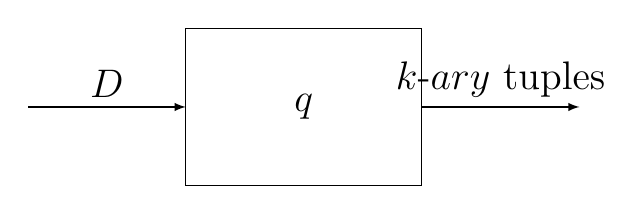
\begin{tikzpicture}
        % Draw the rectangle
        \draw (0,1) rectangle (3,-1) node[midway] {\Large \( q \)};       
        % Draw arrows
        \draw[-latex] (-2,0) -- (0,0) node[midway, above] {\Large \( D \)};
        \draw[-latex] (3,0) -- (5,0) node[midway, above] {\Large \( k\text{-}ary \) tuples};
        \end{tikzpicture}
\end{center}

\begin{itemize}
    \item $D$: Database instance
    \item $k$-ary tuples: tuples with $k$ attributes
    \item $q$: Function on D Over DB $S$
    \item \(q(D)\) is a $k$-ary relation on \(adom(D)\)
\end{itemize}

\remark{\(adom(D)\): the set of all constants appearing in \(D\)}

Q. Given a graph $E$ (binary relation), is the diameter of $E$ at most 3?

\subsection*{Three Fundamental Query Optimization Problems}

1. The Query Satisfiability Problem

Given a query $q$, is there any database instance $D$ such that $q(D) \neq \emptyset$

\begin{verbatim}
    Select *
    from Sells
    where price = 10 and price <>10
\end{verbatim}

$\Rightarrow \emptyset$

2. The Query Equivalence Problem

Given two queries $q$ and $q'$, of the same arity, 
is it the case that $q \equiv q'$? i.e. for every database instance $D$, 
we have that $q(D) = q'(D)$

\begin{verbatim}
Sells(sname, cname, price)
    select sname, cname
    from Sells, Sells
    where Sell.sname = Sells.sname and
        Sells.cname = Sells.cname
=
    Select sname, cname
    From Sells
\end{verbatim}

3. The Query Containment Problem

Given two queries $q$ and $q'$, of the same arity, 
is it the case that $q \subseteq q'$? i.e. for every database instance $D$, 
we have that $q(D) \subseteq q'(D)$

solve 2 can solve 3 or solve 3 can solve 2? (to check)

The question we want to address are:

\begin{enumerate}
    \item How can we measure \textcolor{red}{the precise difficulty} of these problem?
    \item Are there \textcolor{red}{good} algorithms for solving these problems?
    \item If not, any \textcolor{red}{special cases} of these problems for which \textcolor{green}{good} algorithm exist?
\end{enumerate}

\subsection*{Turing}

Ruduction Method is a common way to prove a problem is not recursive aka. undecidable.

\subsubsection*{The Reduction Method}

\( L \leq L^* \) means

\begin{itemize}
    \item It exists a reduction of $L$ to $L^*$
    \item Aka. $L^*$ is at least as hard as $L$
    \item If $L$ is undecidable then $L^*$ is undecidable
    \item This relationship is transitive 
\end{itemize}

\subsection*{Conjunctive Query}

Def. \(\Pi_x(\sigma_\theta(R_1\times...,\times R_n))\),
where $\theta$ is a conjunction of equlity atomic formulas (equijoin)

\begin{verbatim}
    Q(X):- 
\end{verbatim}

\subsubsection*{Homomorphism}

Compress the query to a smaller query

\subsubsection*{Homomorphism between queries}



\subsubsection*{Proof of Homomorphism}

what $c$ stand for of $c(x_1)$? $c$ is mapping

understaind connel database!!

\[Q_1 \in Q_2 \Rightarrow h: Q_2 \rightarrow Q_1\]

\begin{verbatim}
    Q_1(x_1, x_2) :- R(x_1, x_3, x_2), R(x_1, x_3, x_2)
    Q_2(y_1, y_2): R(y_1, y_4, y_2)
\end{verbatim}

\section*{Concurrency}

Transection: A `program' of database operations

\remark{I/O activity can be done in parallel with CPU activity in a computer (cowbook 16.3.1)}

\begin{itemize}
    \item \textcolor{red}{A}tomicity: All actions in the transaction happen or none happen.
    \item \textcolor{red}{C}onsistency: If each transaction is consistent and the database starts in a consistent state before the transaction begins, 
                                        then the database will be consistent when the transaction ends.
    \item \textcolor{red}{I}solation: Execution of a transaction is isolated from other transactions.
    \item \textcolor{red}{D}urability: Once a transaction is committed, its effects persist.
\end{itemize}

\subsection*{Serializability}

\textcolor{red}{Conflict Equivalence} of Two Schedules: 

\begin{enumerate}
    \item They both involve the same set of actions of the same transactions respectively.
    \item The order of every pair of conflicting actions of two transactions is the same in both schedules.
\end{enumerate}

\subsection*{Locking}

Goal of it: 1. Guarantee serializability, 2. preserve high concurrency

Questions to ask:

\begin{itemize}
    \item What \textcolor{red}{modes} of locks to provide?
    \item How to \textbf{get} and \textbf{release} locks? $\Rightarrow$ what sequence, how long?
    \item What units to lock? \(Database \Rightarrow Relation \Rightarrow pages \Rightarrow tuples \Rightarrow attributes\)
\end{itemize}

Unlocking: Release all relevant locks at once or leaf ot root

\newpage
\subsubsection*{Two-Phase Locking}

\begin{itemize}
    \item Growing Phase: A transaction may obtain locks but may not release any lock.
    \item Shrinking Phase: A transaction may release locks but may not obtain any new lock.
\end{itemize}

2PL does not allow the swap of conflicting operations (\(\Rightarrow\) serial order);
and it is possible to swap non-conflicting operations (\(\Rightarrow\) high concurrency)

Problem: it might cause cascading rollback

\begin{figure}[ht]
    \centering
    \includegraphics[width=0.6\textwidth]{./images/cascading_rollback.png}
    \caption{LSNs}
\end{figure}

$T1$ reads the udpated data $A$ of $T2$ and is committed,
but $T2$ is aborted afterwards. $\Rightarrow$ $T1$ must be rolled back, aka. cascading rollback

Solution $\Rightarrow$ strict 2PL (but reduce concurrency)

\subsubsection*{Strict Two-Phase Locking}

\begin{enumerate}
    \item If a transection $T$ wants to read / modify an object, it first requests a shared / exclusive lock on the object.
    \item All locks held by a transaction are released when the transaction is completed.
\end{enumerate}

\remark{A transaction that has an exclusive lock can also read the object.}

state that cannot result from any serial execution of the three transactions

\subsection*{Intention Locks}

\begin{itemize}
    \item Use the put on the parent level to indicate that the child level will be locked
    \item \(IS,IX,SIX\)
\end{itemize}

\remark{SIX allows the read at current level and says that the transaction will write at a lower level.}

Compatibility rule: Reject intention lock if it allows incompatible licks on data items

\subsection*{Degrees of Consistency}

\begin{itemize}
    \item Degree 0: $T$ does not overwite the dirty data of other transactions (short $X$ lock)
    \item Degree 1: $T$ does not commit any writes until the end of the transaction (long $X$ lock)
    \item Degree 2: $T$ does not read dirty data from other transactions (long $X$ lock and short $S$ lock)
    \item Degree 3: Other $T_x$ do not diry any data read by T before T commits (long $X$ lock and long $S$ lock)
\end{itemize}

\section*{Crash Recovery}

\subsection*{Stealing Frames and Forcing Pages}

A page might be written to disk before the transaction $T_1$ is committed. 
E.g. when the buffer pool is full and an another transaction $T_2$ needs to \textbf{bring} in a page, 
the buffer mangeer might choose to replace the frame. ($T_2$ \textcolor{blue}{steals} a frme from $T_1$)

\(\Rightarrow\) need to \textbf{undo} the changes

\remark{Of course, that frame must be unpined by $T_1$, i.e. $T_1$ temporarily does not need the frame.}

After a transaction is committed, all changes of an object has immediately been written to disk.
This is \textcolor{blue}{force} approach

\(\Rightarrow\) need to \textbf{redo} the changes


\subsection*{ARIES}

ARIES is a \textbf{recovery algorithm} designed to work with a steal, no-force approach.

The restart process:

\begin{itemize}
    \item Analysis
    \item Redo
    \item Undo
\end{itemize}

\subsubsection*{The Log}

\subsubsection*{Other Log-Related Structure}

\textbf{1. Transaction Table:} It contains one entry for each active transaction. 
It contains xid, transaction state, \textbf{lastLSN}, and others

\remark{entry: a record for a active transaction.}

\remark{lastLSN: the LSN of the most recent log record for the transaction.}

\textbf{2. Dirty page Table:} It contains one entry for each dirty page in the buffer pool.

The entry contains a field \textbf{rescLSN}, which is the LSN of the first log record that caused the apge to become dirty. 




\subsubsection*{The Write-Ahead Log Protocol}

Two basic rules:

\begin{enumerate}
    \item Before any changes are written to disk, all log records describing these changes MUST first be written to stable storage. (Write)
    \item A transaction cannot be committed until all log records have been written to stable storage. (Ahead)
\end{enumerate}

\begin{figure}[ht]
    \centering
    \includegraphics[width=0.8\textwidth]{./images/lsns.png}
    \caption{LSNs}
\end{figure}

\begin{itemize}
    \item All log records have a unique log sequence number (LSN) which is monotonically increasing.
    \item (In Database) All data page include a page LSN which is the LSN of the last log record that modified the page.
    \item (In RAM) The system keeps tracking of flushedLSN which is the largest LSN of all log records that have been written to disk.
\end{itemize}

The \(pageLSN \leq flushedLSN\) is the core rule of WAL, ensuring that all log records are written to disk before the corresponding data pages.
$\Rightarrow$ keep data consistent and recoverable.

\section{}

\section*{TO TA/Professor}

\begin{itemize}
    \item why in 2 pass merge sort the number of M unit increases?
    \item book 9.7 why to point free space there?
    \item why not small relation in memory and scan the large relation and join $\Rightarrow O(T(S)B(R))$ 
    \item for clustered relation, Index nested loops is better than Optimized Two-pass multi-way merge sort?
\end{itemize}

\end{document}